\documentclass[a4paper]{article}

% --- UNIVERSAL PREAMBLE BLOCK ---
\usepackage[a4paper, top=1.5cm, bottom=1.5cm, left=1.5cm, right=1.5cm]{geometry}
\usepackage{fontspec}

\usepackage[indonesian, provide=*]{babel}
\babelprovide[import, onchar=ids fonts]{indonesian}
\babelprovide[import, onchar=ids fonts]{english}

% Set default/Latin font to Sans Serif (Noto Sans)
\babelfont{rm}{Noto Sans}
\babelfont{sf}{Noto Sans}

% Packages for graphics and layout
\usepackage{tikz}
\usetikzlibrary{shapes, shapes.symbols, arrows.meta, positioning, calc, shadows, backgrounds, patterns, decorations.pathreplacing}
\usepackage[most]{tcolorbox}
\usepackage{multicol}
\usepackage{enumitem}

% --- COLOR DEFINITIONS (SAME AS SOURCE) ---
\definecolor{mainBlue}{HTML}{2C3E50}
\definecolor{accentTeal}{HTML}{16A085}
\definecolor{alertRed}{HTML}{E74C3C}
\definecolor{niceOrange}{HTML}{F39C12}
\definecolor{powerBlue}{HTML}{2980B9}
\definecolor{cubeRed}{HTML}{C0392B}
\definecolor{softBgA}{HTML}{ECF0F1}
\definecolor{softBgB}{HTML}{F7F9F9}
\definecolor{solGreen}{HTML}{27AE60}
\definecolor{lightPurple}{HTML}{9B59B6}

% --- CUSTOM BAR MODEL COMMANDS ---

% Standard Bar Segment
\newcommand{\DrawBarSegment}[4]{
    % #1: x, #2: y, #3: width, #4: color
    \draw[fill=#4!20, draw=mainBlue, thick] (#1, #2) rectangle (#1+#3, #2+1);
}

% Brace Command
\newcommand{\DrawBraceDown}[4]{
    % #1: start x, #2: end x, #3: y level, #4: Label
    \draw[decorate, decoration={brace, mirror, amplitude=5pt}, thick, mainBlue] (#1, #3) -- (#2, #3) node[midway, below=7pt, font=\small\bfseries] {#4};
}

\newcommand{\DrawBraceUp}[4]{
    % #1: start x, #2: end x, #3: y level, #4: Label
    \draw[decorate, decoration={brace, amplitude=5pt}, thick, mainBlue] (#1, #3) -- (#2, #3) node[midway, above=7pt, font=\small\bfseries] {#4};
}

\newcommand{\checkbox}{\tikz[baseline=-0.6ex]{\draw[thick, mainBlue] (0,0) rectangle (0.3,0.3);}}

% --- CUSTOM BOX FOR CONCEPTS ---
\newtcolorbox{ConceptBox}[2][]{
    enhanced,
    colback=white,
    colframe=mainBlue!20!white,
    boxrule=0.5pt,
    left=2mm, right=2mm, top=2mm, bottom=2mm,
    title={\textbf{#2}},
    coltitle=mainBlue,
    fonttitle=\bfseries\large,
    attach boxed title to top left={yshift=-2mm, xshift=2mm},
    boxed title style={boxrule=0pt, colframe=white, colback=white},
    #1
}

\begin{document}

% =================================================================================
% PART 1: INTRODUCTION & CONTEXT
% =================================================================================

\tikzset{
    arrowFlow/.style={->, >={Latex[width=3mm,length=3mm]}, ultra thick, draw=accentTeal},
    conceptBox/.style={
        rectangle, rounded corners, draw=none, fill=white, drop shadow,
        text width=4.5cm, align=center, minimum height=2cm, font=\small
    }
}

% --- HEADER ---
\begin{tcolorbox}[colback=mainBlue, colframe=mainBlue, arc=0mm, boxrule=0pt, top=5mm, bottom=5mm, halign=center]
    {\Huge \bfseries \color{white} SINGAPORE BAR MODEL} \\
    \vspace{0.2cm}
    {\large \color{accentTeal} \textbf{Jembatan Visual Soal Cerita ke Aljabar}}
\end{tcolorbox}

\vspace{0.2cm}

% --- SECTION 1: KONTEKS MASALAH & SOLUSI ---
\begin{tcolorbox}[title=\textbf{1. FILOSOFI: MENGAPA BAR MODEL?}, colback=white, colframe=lightPurple, coltitle=white, fonttitle=\bfseries\large]
    \begin{minipage}[t]{0.48\textwidth}
        \textcolor{alertRed}{\Large \textbf{A. Masalah: "Lost in Translation"}}
        \vspace{0.1cm}
        \begin{itemize}[leftmargin=*, itemsep=2pt]
            \item \textbf{Abstraksi Dini:} Siswa kesulitan langsung mengubah kalimat cerita menjadi persamaan matematika ($x + y = z$).
            \item \textbf{Struktur Tersembunyi:} Hubungan antar besaran (lebih banyak, selisih, total) tidak terlihat dalam teks.
        \end{itemize}
    \end{minipage}%
    \hfill
    \begin{minipage}[t]{0.48\textwidth}
        \textcolor{accentTeal}{\Large \textbf{B. Solusi: Representasi Piktorial}}
        \vspace{0.1cm}
        \begin{itemize}[leftmargin=*, itemsep=2pt]
            \item \textbf{Visualisasi Kuantitas:} Panjang batang merepresentasikan nilai (magnitude).
            \item \textbf{Visualisasi Relasi:} Posisi batang (berderet atau bertumpuk) menunjukkan hubungan penjumlahan atau perbandingan.
        \end{itemize}
    \end{minipage}
\end{tcolorbox}

% --- SECTION 2: ANATOMI ---
\begin{tcolorbox}[title=\textbf{2. ANATOMI BAR MODEL}, colback=white, colframe=accentTeal, coltitle=white, fonttitle=\bfseries\large]
    \centering
    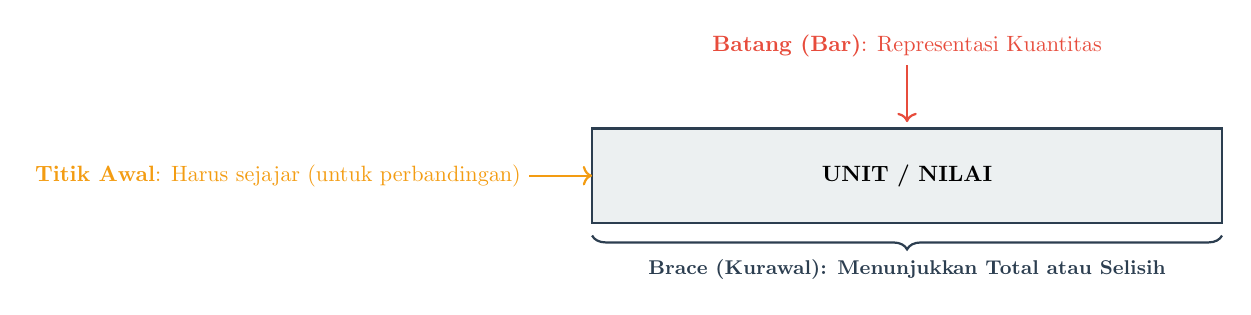
\begin{tikzpicture}[scale=0.8, transform shape]
        % Main Bar
        \draw[fill=softBgA, draw=mainBlue, thick] (0,0) rectangle (10, 1.5);
        
        % Labels inside
        \node at (5, 0.75) {\textbf{UNIT / NILAI}};
        
        % Anatomy annotations
        \draw[<-, thick, alertRed] (5, 1.6) -- (5, 2.5) node[above] {\textbf{Batang (Bar)}: Representasi Kuantitas};
        \draw[<-, thick, niceOrange] (0, 0.75) -- (-1, 0.75) node[left] {\textbf{Titik Awal}: Harus sejajar (untuk perbandingan)};
        
        % Brace
        \DrawBraceDown{0}{10}{-0.2}{Brace (Kurawal): Menunjukkan Total atau Selisih}
    \end{tikzpicture}
    \vspace{0.2cm} \hrule \vspace{0.2cm}
    \begin{minipage}{0.9\textwidth}
        \textbf{Prinsip Dasar:}
        \begin{itemize}[leftmargin=*, label=\checkbox]
            \item \textbf{Panjang Proporsional:} Nilai yang lebih besar digambar lebih panjang (sketsa, tidak perlu presisi milimeter).
            \item \textbf{Konservasi:} Batang bisa dipotong, digeser, atau digabung tanpa mengubah nilai totalnya.
        \end{itemize}
    \end{minipage}
\end{tcolorbox}

% --- SECTION 3: C-P-A BRIDGE ---
\begin{tcolorbox}[title=\textbf{3. TRANSISI C-P-A (PENGENALAN ALJABAR)}, colback=softBgA, colframe=niceOrange, coltitle=white, fonttitle=\bfseries\large]
    \centering
    \begin{tikzpicture}[node distance=0.2cm and 0.5cm]
        \node[conceptBox] (concrete) {
            \textbf{A. KONKRET}\\ \textit{3 Keranjang "x"}\\ \vspace{0.1cm}
            \begin{tikzpicture}[scale=0.4, baseline=0] 
                % Basket 1
                \begin{scope}[shift={(0,0)}]
                    \draw[thick, mainBlue] (0.1,0.2) to[out=110, in=70] (1.4,0.2);
                    \draw[fill=niceOrange!40, draw=mainBlue, thick] (0,0.2) -- (0.25,-0.6) -- (1.25,-0.6) -- (1.5,0.2) -- cycle;
                    \node[font=\bfseries\large, mainBlue] at (0.75, -0.2) {$x$};
                \end{scope}
                % Basket 2
                \begin{scope}[shift={(1.8,0)}]
                    \draw[thick, mainBlue] (0.1,0.2) to[out=110, in=70] (1.4,0.2);
                    \draw[fill=niceOrange!40, draw=mainBlue, thick] (0,0.2) -- (0.25,-0.6) -- (1.25,-0.6) -- (1.5,0.2) -- cycle;
                    \node[font=\bfseries\large, mainBlue] at (0.75, -0.2) {$x$};
                \end{scope}
                % Basket 3
                \begin{scope}[shift={(3.6,0)}]
                    \draw[thick, mainBlue] (0.1,0.2) to[out=110, in=70] (1.4,0.2);
                    \draw[fill=niceOrange!40, draw=mainBlue, thick] (0,0.2) -- (0.25,-0.6) -- (1.25,-0.6) -- (1.5,0.2) -- cycle;
                    \node[font=\bfseries\large, mainBlue] at (0.75, -0.2) {$x$};
                \end{scope}
            \end{tikzpicture}
        };
        \node[conceptBox, right=of concrete] (pictorial) {
            \textbf{B. PIKTORIAL}\\ \textit{3 Himpunan Variabel}\\ \vspace{0.1cm}
            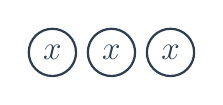
\begin{tikzpicture}[scale=0.5, baseline=-5] 
                % Circle 1
                \draw[thick, mainBlue, fill=white] (0, 0) circle (0.6);
                \node[font=\bfseries\large, mainBlue, anchor=center] at (0, 0) {$x$};
                
                % Circle 2
                \draw[thick, mainBlue, fill=white] (1.5, 0) circle (0.6);
                \node[font=\bfseries\large, mainBlue, anchor=center] at (1.5, 0) {$x$};
                
                % Circle 3
                \draw[thick, mainBlue, fill=white] (3.0, 0) circle (0.6);
                \node[font=\bfseries\large, mainBlue, anchor=center] at (3.0, 0) {$x$};
            \end{tikzpicture}
        };
        \node[conceptBox, right=of pictorial] (abstract) {
            \textbf{C. ABSTRAK}\\ \textit{Aljabar}\\ \vspace{0.1cm}
            \tikz{\node[font=\bfseries\Huge, color=mainBlue] {3x};}
        };
        \draw[arrowFlow] (concrete) -- (pictorial); 
        \draw[arrowFlow] (pictorial) -- (abstract);
    \end{tikzpicture}
\end{tcolorbox}

\newpage

% =================================================================================
% PART 2: TIPE STRUKTUR DASAR (CORE THEORY)
% =================================================================================

\tikzset{
    modelLabel/.style={font=\bfseries\small, color=mainBlue},
    questionMark/.style={font=\bfseries\large, color=alertRed}
}

% --- HEADER PART 2 ---
\begin{tcolorbox}[colback=mainBlue, colframe=mainBlue, arc=0mm, boxrule=0pt, top=4mm, bottom=4mm, halign=center]
    {\Huge \bfseries \color{white} STRUKTUR DASAR} \\
    \vspace{0.1cm}
    {\large \color{accentTeal} \textbf{Empat Logika Utama Bar Model}}
\end{tcolorbox}
\vspace{0.3cm}

% --- TYPE 1: PART-WHOLE ---
\begin{ConceptBox}{TIPE 1: PART-WHOLE MODEL (Bagian-Keseluruhan)}
\begin{minipage}{0.45\textwidth}
    \centering
    \begin{tikzpicture}[scale=0.7]
        % Whole Bar split into two
        \draw[fill=accentTeal!30, draw=mainBlue, thick] (0,0) rectangle (4, 1.5);
        \draw[fill=niceOrange!30, draw=mainBlue, thick] (4,0) rectangle (7, 1.5);
        
        % Labels
        \node[modelLabel] at (2, 0.75) {Bagian A};
        \node[modelLabel] at (5.5, 0.75) {Bagian B};
        
        % Braces
        \DrawBraceUp{0}{7}{1.6}{TOTAL (WHOLE)}
        \node[font=\tiny, below] at (2,0) {Diketahui / Ditanya};
        \node[font=\tiny, below] at (5.5,0) {Diketahui / Ditanya};
    \end{tikzpicture}
\end{minipage}%
\hfill
\begin{minipage}{0.5\textwidth}
    \textbf{Kapan Digunakan?}
    \begin{itemize}[leftmargin=*, itemsep=2pt]
        \item Operasi Penjumlahan (Mencari Total).
        \item Operasi Pengurangan (Diketahui Total dan satu Bagian, mencari Bagian lain).
        \item Tidak ada perbandingan "lebih banyak/sedikit".
    \end{itemize}
    \textit{Contoh Kalimat: "A dan B digabungkan...", "Sebagian adalah A, sisanya B..."}
\end{minipage}
\end{ConceptBox}

\vspace{0.3cm}

% --- TYPE 2: COMPARISON ---
\begin{ConceptBox}{TIPE 2: COMPARISON MODEL (Perbandingan)}
\begin{minipage}{0.45\textwidth}
    \centering
    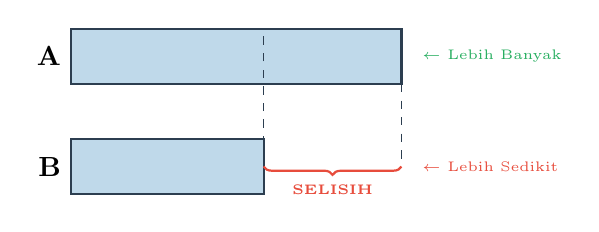
\begin{tikzpicture}[scale=0.7]
        % Bar A
        \node[left, font=\bfseries] at (0, 2.5) {A};
        \draw[fill=powerBlue!30, draw=mainBlue, thick] (0,2) rectangle (6, 3);
        
        % Bar B (Shorter)
        \node[left, font=\bfseries] at (0, 0.5) {B};
        \draw[fill=powerBlue!30, draw=mainBlue, thick] (0,0) rectangle (3.5, 1);
        
        % Dotted lines for comparison
        \draw[dashed, mainBlue] (3.5, 0) -- (3.5, 3);
        \draw[dashed, mainBlue] (6, 2) -- (6, 0.5);
        
        % Difference Brace
        \draw[decorate, decoration={brace, mirror, amplitude=3pt}, thick, alertRed] (3.5, 0.5) -- (6, 0.5) node[midway, below=3pt, font=\bfseries\tiny] {SELISIH};
        
        % Comparison logic - MOVED TO THE RIGHT TO AVOID COLLISION
        \node[font=\tiny, anchor=west, text=solGreen] at (6.2, 2.5) {$\leftarrow$ Lebih Banyak};
        \node[font=\tiny, anchor=west, text=alertRed] at (6.2, 0.5) {$\leftarrow$ Lebih Sedikit};
    \end{tikzpicture}
\end{minipage}%
\hfill
\begin{minipage}{0.5\textwidth}
    \textbf{Kapan Digunakan?}
    \begin{itemize}[leftmargin=*, itemsep=2pt]
        \item Membandingkan dua entitas berbeda.
        \item Kata kunci: "Lebih banyak dari", "Lebih sedikit dari", "Berapa bedanya", "Sama banyak dengan".
    \end{itemize}
    \textbf{Konsep Kunci:} Alignment (Kesejajaran) di sisi kiri sangat krusial untuk melihat selisih di sisi kanan.
\end{minipage}
\end{ConceptBox}

\vspace{0.3cm}

% --- TYPE 3: EQUAL PARTS / MULTIPLICATION ---
\begin{ConceptBox}{TIPE 3: EQUAL PARTS (Perkalian \& Pembagian)}
\begin{minipage}{0.45\textwidth}
    \centering
    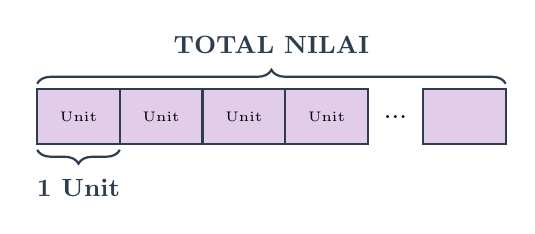
\begin{tikzpicture}[scale=0.7]
        % Bar split into equal parts
        \foreach \x in {0, 1.5, 3, 4.5} {
            \draw[fill=lightPurple!30, draw=mainBlue, thick] (\x, 0) rectangle (\x+1.5, 1);
            \node[font=\tiny] at (\x+0.75, 0.5) {Unit};
        }
        
        % Dot dot dot implies many
        \node at (6.5, 0.5) {...};
        \draw[fill=lightPurple!30, draw=mainBlue, thick] (7, 0) rectangle (8.5, 1);
        
        % Braces
        \DrawBraceDown{0}{1.5}{-0.1}{1 Unit}
        \DrawBraceUp{0}{8.5}{1.1}{TOTAL NILAI}
        
    \end{tikzpicture}
\end{minipage}%
\hfill
\begin{minipage}{0.5\textwidth}
    \textbf{Kapan Digunakan?}
    \begin{itemize}[leftmargin=*, itemsep=2pt]
        \item Benda-benda identik dalam jumlah banyak.
        \item Pecahan (Fraction): 1 bagian dari 5 bagian yang sama.
        \item Rasio (Perbandingan Senilai): 3 kotak vs 2 kotak.
    \end{itemize}
    \textbf{Konsep Kunci:} "Unitary Method". Mencari nilai \textbf{1 Unit} adalah kunci untuk memecahkan seluruh masalah.
\end{minipage}
\end{ConceptBox}

\vspace{0.3cm}

% --- TYPE 4: BEFORE-AFTER / CHANGE ---
\begin{ConceptBox}{TIPE 4: CHANGE MODEL (Perubahan/Transformasi)}
\begin{minipage}{0.45\textwidth}
    \centering
    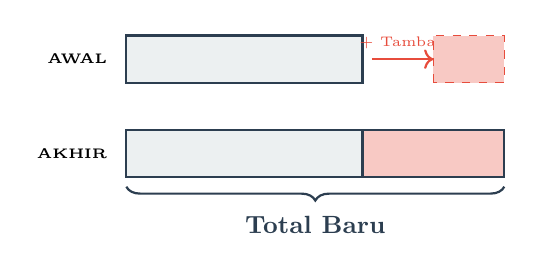
\begin{tikzpicture}[scale=0.6]
        % Before
        \node[anchor=east, font=\bfseries\tiny] at (-0.2, 2.5) {AWAL};
        \draw[fill=softBgA, draw=mainBlue, thick] (0,2) rectangle (5, 3);
        
        % Operation Arrow
        \draw[->, thick, alertRed] (5.2, 2.5) -- (6.5, 2.5) node[midway, above, font=\tiny] {+ Tambah};
        \draw[fill=alertRed!30, draw=alertRed, dashed] (6.5, 2) rectangle (8, 3);
        
        % After
        \node[anchor=east, font=\bfseries\tiny] at (-0.2, 0.5) {AKHIR};
        \draw[fill=softBgA, draw=mainBlue, thick] (0,0) rectangle (5, 1);
        \draw[fill=alertRed!30, draw=mainBlue, thick] (5,0) rectangle (8, 1);
        
        % Brace showing new total
        \DrawBraceDown{0}{8}{-0.2}{Total Baru}
    \end{tikzpicture}
\end{minipage}%
\hfill
\begin{minipage}{0.5\textwidth}
    \textbf{Kapan Digunakan?}
    \begin{itemize}[leftmargin=*, itemsep=2pt]
        \item Situasi dinamis (ada aksi).
        \item "Memberi", "Menerima", "Menjual", "Memakan".
    \end{itemize}
    \textbf{Konsep Kunci:} Visualisasikan proses penambahan (memperpanjang batang) atau pengurangan (memotong/mencoret batang).
\end{minipage}
\end{ConceptBox}

\end{document}
